% !TEX root = ../main.tex

LoopWAM learns a world--action model that can be updated with experience collected during deployment.
The framework couples video and action generation within a shared denoising process, then uses trajectory quality to distinguish how deployment data supervise world modeling and control.
Figure~\ref{fig:method} summarizes the architecture and training procedure.
We first introduce joint world--action modeling, followed by quality-aware learning from mixed trajectories and the deployment--learning loop.

\begin{figure}[t]
    \centering
    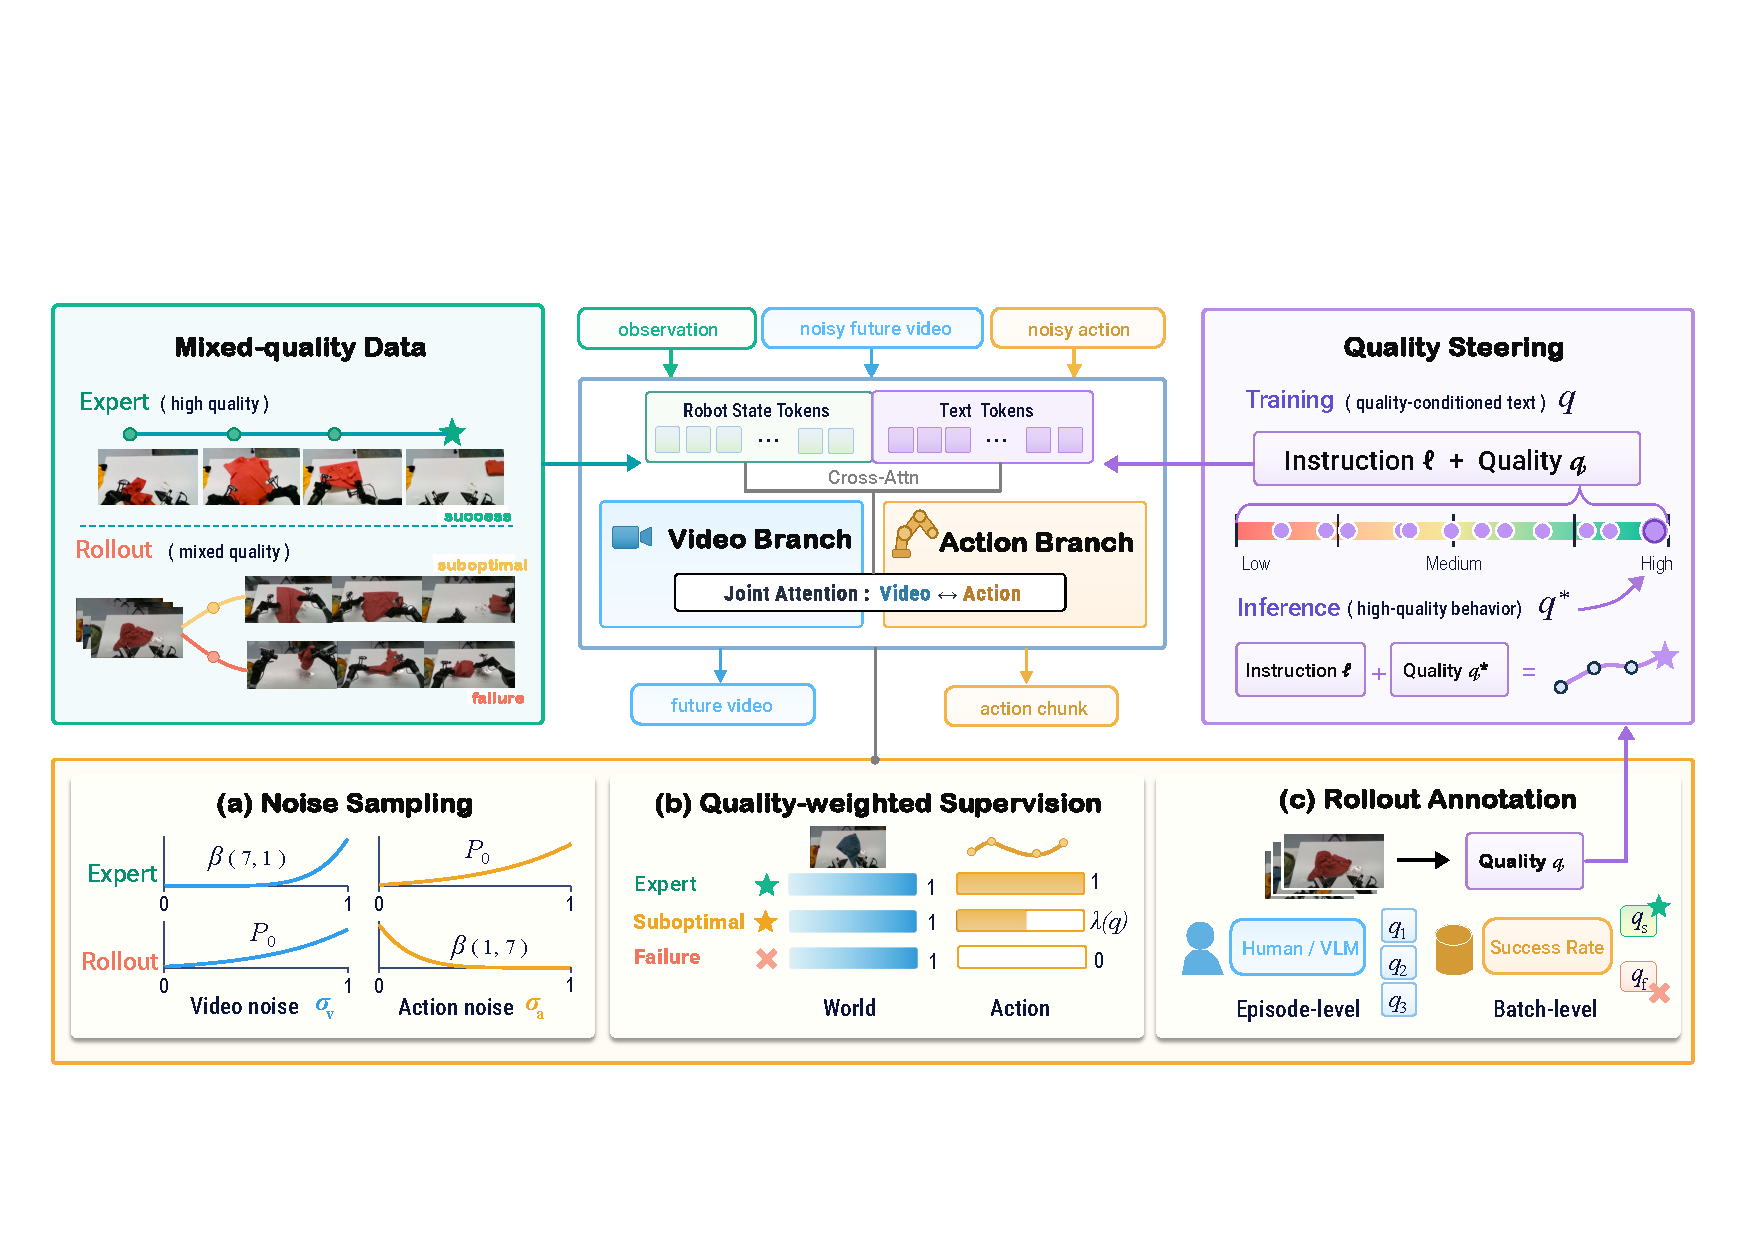
\includegraphics[width=\linewidth,pagebox=cropbox]{figures/LoopWAM_method0926.pdf}
    \caption{\textbf{Overview of LoopWAM.}
    LoopWAM is structured as a Mixture-of-Transformer (MoT) architecture, where bidirectional attention enables feature interaction between the video and action branches.
    Training combines quality-conditioned instructions, source-dependent noise sampling, and quality-weighted action supervision.
    Expert trajectories supervise both modalities, while lower-quality rollouts retain full world supervision and contribute to action imitation according to their quality.
    The trained model is deployed using the expert score $q^\star$, and recorded experience returns to the next training round.}
    \label{fig:method}
\end{figure}

\subsection{Joint World--Action Modeling}
\label{sec:coupled_model}

We consider language-conditioned manipulation with visual observation $o_t$, robot state $s_t$, and instruction $\ell$.
The prediction targets are an action chunk $A_t=(a_t,\ldots,a_{t+H-1})$ and the corresponding future observations $V_t$, sampled over the same horizon.
A pretrained video VAE maps $(o_t,V_t)$ to an observation latent $z_o$ and future latents $Z_t$.
LoopWAM models their joint distribution
\begin{equation}
    p_\theta(A_t,Z_t\mid o_t,s_t,\ell,q),
    \label{eq:quality_joint}
\end{equation}
where $q$ is a numerical score of trajectory quality, as detailed in Section~\ref{sec:quality_steering}.
This unified formulation enables a single model to learn action generation and visual dynamics from paired action--observation sequences~\citep{zhu2025unifiedworldmodelscoupling}.

We instantiate this formulation with a dual-stream diffusion transformer whose video backbone is initialized from Wan2.2-TI2V-5B~\citep{wan2025}.
The video and action streams have separate token projections, transformer parameters, and prediction heads, with joint attention connecting the streams at every layer.
To train them with flow matching~\citep{lipman2023flow}, we independently perturb each target $X_m$, where $X_v=Z_t$ and $X_a=A_t$:
\begin{equation}
    X_m^{\sigma_m}=(1-\sigma_m)X_m+\sigma_m\epsilon_m,
    \qquad \epsilon_m\sim\mathcal N(0,I),\quad m\in\{v,a\}.
    \label{eq:flow_path}
\end{equation}
The joint network predicts velocity fields $(v_\theta^v,v_\theta^a)$ with targets $u_m=\epsilon_m-X_m$.
Each stream receives noise level $\sigma_m$, with $0$ denoting clean data and $1$ pure noise; the observation latent $z_o$ remains clean.

The attention structure couples the two predictions throughout denoising.
Denote observation, future-video, and action tokens by $O$, $V$, and $A$, respectively.
Their block mask, with queries indexing rows and keys indexing columns, is
\begin{equation}
    M_{(O,V,A)}=
    \begin{pmatrix}
        1 & 0 & 0\\
        1 & 1 & 1\\
        1 & 1 & 1
    \end{pmatrix},
    \label{eq:joint_mask}
\end{equation}
where $1$ permits attention.
Observation tokens attend only within the initial frame.
Both streams cross-attend to the quality-conditioned instruction; robot-state tokens additionally condition the action stream.
Together with the training scheme in Section~\ref{sec:quality_steering}, this architecture supports learning both embodied world representations and awareness of action consequences.
Dense video supervision on expert and mixed-quality rollouts broadens the interactions from which these representations are learned.
Through bidirectional attention, the world-prediction loss also trains features used for action generation.
This training couples learning how tasks can be completed with learning how particular actions affect their outcomes, encouraging consistency between video and action generation.
% AUTHOR CHECK: The stated conditioning split matches both README training
% commands (video_cross_attend_proprio=false). The snapshot's inherited
% infer_action() / _predict_joint_noise() path instead shares a text-plus-state
% context. Confirm the actual deployment implementation before submission.

\subsection{Quality-Aware Learning from Mixed Trajectories}
\label{sec:quality_steering}

Our training corpus combines expert demonstrations $\mathcal D_E$ with rollout data $\mathcal D_R$ of arbitrary quality, including successful, suboptimal, and failed executions.
These rollouts substantially broaden the state--action--outcome distribution beyond expert paths, providing world-model supervision even when their actions are undesirable imitation targets.
Each trajectory is assigned a source indicator $d\in\{E,R\}$; every training segment extracted from that trajectory uses the same indicator.
We combine source-dependent noise sampling, quality conditioning, and selective action supervision to learn from this broader experience while favoring high-quality behavior.

\textbf{Source-dependent noise sampling.}
\label{sec:noise_sampling}
Jointly predicting video and actions in a WAM does not by itself ensure that the predicted futures reflect the consequences of the generated actions.
To improve consistency between video and action generation and make world predictions more useful for control, we aim to strengthen action-conditioned world modeling (ACWM) within the same unified model.
We therefore use source-dependent noise sampling to make recorded rollout actions accessible when predicting their observed consequences, while retaining joint video--action generation in a single training stage.
Specifically, we select different noise distributions for expert and rollout segments, while drawing video and action noise levels independently within each segment:
\begin{equation}
\begin{aligned}
    d=E:&\quad \sigma_v\sim\operatorname{Beta}(7,1),
                 &&\sigma_a\sim\mathcal P_0,\\
    d=R:&\quad \sigma_v\sim\mathcal P_0,
                 &&\sigma_a\sim\operatorname{Beta}(1,7).
\end{aligned}
\label{eq:source_noise}
\end{equation}
Here $\mathcal P_0$ is the base noise distribution obtained by sampling $u\sim\mathcal U(0,1)$ and setting $\sigma=\phi_\kappa(u)=\kappa u/[1+(\kappa-1)u]$, with $\kappa=5$.
The Beta distributions~\citep{johnson1995continuous} are applied directly to $\sigma$.
For expert data, high video noise emphasizes recovering expert futures from strongly corrupted inputs, alongside action generation over the base noise distribution.
For rollouts, low action noise preserves much of the recorded motion while the video stream predicts its visual consequences.
Training across these executions broadens the action--outcome distribution seen by the world model, including transitions in which the task remains incomplete or an interaction fails.
Joint attention then connects this consequence-learning signal to the representations used for action generation.

\textbf{Quality steering.}
Within this unified training scheme, each trajectory is assigned a numerical quality score $q$, which is shared by all training segments extracted from it.
We encode quality as a suffix to the instruction, $\ell_q=[\ell;\texttt{Quality:}\ q]$, and use its text embeddings to condition both video and action streams.
We support two trajectory annotation schemes: (1) \emph{Episode-level annotation}, where human annotators or a vision-language model (VLM) score each trajectory individually for fine-grained quality estimation; and (2) \emph{coarse-level annotation}, where a single human-provided score is assigned to all rollouts from a policy checkpoint based on its overall success rate and motion smoothness.
Under coarse annotation, successful trajectories receive the checkpoint score while failed trajectories receive the minimum score, requiring only one annotation per checkpoint.
Both schemes represent rollout quality using numerical scores.
For expert demonstrations, we assign an expert score $q^\star$ that is higher than the maximum rollout quality score.
The quality-conditioned instruction allows different behaviors under the same task instruction to be represented within one model.
During deployment, we condition on $q=q^\star$ to steer sampling toward expert-quality behavior.

\textbf{Quality-weighted supervision.}
\label{sec:quality_objective}
Given these noise levels and quality scores, we retain video prediction on all trajectory qualities and modulate action supervision with a nondecreasing weight $\lambda(q)\in[0,1]$.
Expert trajectories receive full action supervision with $\lambda(q^\star)=1$, while failed trajectories use $\lambda(q)=0$ and receive no action supervision.
For sample $i$ and modality $m$, define the denoising loss
\begin{equation}
    \ell_{m,i}=\omega(\sigma_{m,i})
    \left\|v_{\theta,i}^{m}-(\epsilon_{m,i}-X_{m,i})\right\|_{\mathrm{valid}}^2,
    \label{eq:modality_loss}
\end{equation}
where the norm denotes mean squared error over valid target elements and $\omega$ is the common timestep weighting function.
The clean observation latent is excluded from video supervision, and padded targets are masked in both modalities.
For a minibatch of $B$ segments, the complete objective is
\begin{equation}
    \mathcal L_{\mathrm{LoopWAM}}
    =\underbrace{\frac{1}{B}\sum_{i=1}^{B}\ell_{v,i}}_{\text{world supervision}}
    +\underbrace{\frac{\sum_{i=1}^{B}\lambda(q_i)\ell_{a,i}}
        {\max\!\left(1,\sum_{i=1}^{B}\lambda(q_i)\right)}}_{\text{quality-weighted action supervision}}.
    \label{eq:quality_loss}
\end{equation}
The source indicator determines corruption, whereas quality controls the behavior condition and action weight.
In particular, $\lambda(q)=0$ removes direct imitation of a trajectory's actions while preserving world-model gradients through the jointly attended video and action representations.
Quality steering and weighted supervision thus allow broader transition learning while concentrating action imitation on more desirable behavior.
The data preprocessing are specified in Appendix~\ref{app:implementation}.

\subsection{Closed-Loop Self-Improvement}
\label{sec:deployment_loop}

The deployed policy uses the high-quality action marginal of the joint model:
\begin{equation}
    \pi_\theta(A_t\mid o_t,s_t,\ell;q^\star)
    =\int p_\theta(A_t,Z_t\mid o_t,s_t,\ell,q^\star)\,\mathrm d Z_t.
    \label{eq:steered_policy}
\end{equation}
In practice, we sample this marginal by jointly denoising video and actions from Gaussian noise, holding the current observation latent fixed.
% Both streams follow Euler integration from $\sigma=1$ to $0$.
% The robot executes the generated actions and conditions subsequent predictions on newly acquired observations; future-video latents participate in action generation even when pixel-space decoding is omitted.
Starting from an expert-trained model, we collect and score deployment rollouts, then update the model on expert demonstrations and all accumulated rollouts using Equation~\ref{eq:quality_loss}.
Each updated model is redeployed with the expert score $q^\star$ to continue the deployment--learning loop.

More broadly, LoopWAM's self-improvement updates can use rollouts from arbitrary deployed policies, even poorly performing ones.
The joint architecture and quality-aware objective accommodate their varying trajectory qualities, so each trajectory contributes according to its observed transitions and behavioral quality.
This extends self-improvement to learning from deployment experience collected by other policies as well as LoopWAM itself.
We validate this broader setting on RoboTwin~2.0 and RoboCasa365 (Section~\ref{sec:benchmark_results}).
